\documentclass[cn,hazy,green,12pt,normal]{elegantnote}

\title{作业1解答}
\author{24Spring 回归分析}
\date{\today}

\usepackage{array}

\usepackage{amsmath, amssymb, bm, color, framed, graphicx, hyperref, mathrsfs, fontspec, geometry, extarrows, amsthm}

\DeclareMathOperator{\e}{\!\!\;\mathrm e}
\DeclareMathOperator{\Cov}{Cov}
\DeclareMathOperator{\Var}{Var}
\DeclareMathOperator{\var}{var}
\DeclareMathOperator{\tr}{tr}
\DeclareMathOperator{\diag}{diag}
\newcommand{\p}{\partial}
\renewcommand{\d}{\mathop{}\!\mathrm{d}}
\newcommand{\MR}{\mathbb R}
\newcommand{\MC}{\mathbb C}
\newcommand{\MF}{\mathbb F}
\newcommand{\MZ}{\mathbb Z}
\newcommand{\MN}{\mathbb N}
\newcommand{\MCF}{\mathscr F}
\renewcommand{\Re}{\operatorname{Re}}
\renewcommand{\Im}{\operatorname{Im}}
\renewcommand{\boldsymbol}{\bm}
\renewcommand{\i}{\mathrm i}

\DeclareMathOperator{\Arg}{Arg}
\DeclareMathOperator{\I}{I}
\usepackage{tkz-euclide}
\numberwithin{equation}{section}
\numberwithin{subsection}{section}

\lstset{
    language=R,
    basicstyle=\ttfamily,
    keywordstyle=\color{blue},
    commentstyle=\color{gray},
    frame=single,
    breaklines=true
}

\begin{document}
\maketitle
\begin{homework}
    假设一物体长度为$\mu$,但$\mu$未知,我们欲估计它,于是将其测量了n次,得到测量值为$y_1,y_2,\dots,y_n$。如果测量过程没有系统误差,我们可以认为$y_i,i=1,\dots,n$为来自正态总体$N(\mu,\sigma^2)$的一组随机样本。试将这些数据表示成线性模型形式。
\end{homework}

\begin{proof}[\solutionname]
    \[ 
    \bm y= \begin{bmatrix}
        y_1\\
        \vdots\\
        y_n
    \end{bmatrix}\quad
    \bm y=\mu \bm 1 + \bm \e \quad
    \bm \e \sim N(\bm 0, \sigma^2 I_n)
    \]
\end{proof}

\begin{note}
    误差项的Gauss-Markov假设
\end{note}

\begin{homework}
    下面的模型是否为一般线性模型?如果不是,能否通过适当的变换使之成为线性模型?

    (1)$Y=\beta_0+\beta_1X_1+\beta_2X_1^2+\beta_3lnX_2+\epsilon$

    (2)$Y=\epsilon \,exp(\beta_0+\beta_1X_1+\beta_2X_1^2)$

    (3)$Y=[1+exp(\beta_0+\beta_1X_1+\epsilon)]^{-\frac{1}{2}}$

    (4)$Y=\beta_0+\beta_1(X_1+X_2)+\beta_2e^{X_1+X_2}+\beta_3lnX_1^2+\epsilon$
\end{homework}
\begin{proof}[\solutionname]
    (1)是。

    (2)不是,两侧取绝对值,再取对数,令$\tilde{Y}=ln |Y|,\tilde{\epsilon}=ln|\epsilon|,\tilde{X_2}=X_1^2$变换为线性模型.

    (3)不是,先两侧平方,取倒数,同时减1,再取对数。令$\tilde{Y}=ln(Y^{-2}-1)$得。
\end{proof}

(4)是。

\begin{note}
    重点看是否对参数线性。
\end{note}

\begin{homework}
    写出二元线性回归模型,并参考教学课件第一章第一节p20 Table1.1中矫正叉积矩阵符号给出回归系数的最小二乘(OLS)估计。
\end{homework}
\begin{proof}[\solutionname]
\[
    \bm y = \alpha \bm 1_n+X_c \bm \beta_c +\bm e
    \]
    其中p=3。由公式得$\hat{\alpha}=\Bar{y}$,$\hat{\bm \beta_c}=(X_c^TX_c)^{-1}X_c^T\bm y$,
    \[
    \hat{\bm \beta_c}=
    \begin{bmatrix}
        SX_1X_1&SX_1X_2\\
        SX_2X_1&SX_2X_2\\
    \end{bmatrix}^{-1}\begin{bmatrix}
        (X_1-\bm 1 m_1)^T\\
        (X_2-\bm 1 m_2)^T\\
    \end{bmatrix}\bm y
    =\begin{bmatrix}
        SX_1X_1&SX_1X_2\\
        SX_2X_1&SX_2X_2\\
    \end{bmatrix}^{-1}\begin{bmatrix}
        SX_1Y\\
        SX_2Y
    \end{bmatrix}\]
\end{proof}

\begin{homework}
    为考察某种维尼纶纤维的耐水性,安排了一批实验,测得甲醛浓度X及"浓缩化度"Y的数据如下:
    
\begin{tabular}{|l|l|l|l|l|l|l|l|}
\hline
X & 18    & 20    & 22    & 24    & 26    & 28 & 30    \\ \hline
Y & 26.86 & 28.35 & 28.75 & 28.87 & 29.75 & 30 & 30.36 \\ \hline
\end{tabular}

从实际经验及理论知识假设两者近似线性关系。求Y关于X的OLS拟合回归方程,并借助R或Python画出散点图和拟合回归直线。
\end{homework}
\begin{proof}[\solutionname]

\begin{lstlisting}
x <- seq(18, 30, by=2)
y <- c(26.86, 28.35, 28.75, 28.87, 29.75, 30, 30.36)
model <- lm(y ~ x)
plot(x, y, xlab = "X", ylab = "Y")  # draw a picture
abline(model)
summary(model)  # view details
    \end{lstlisting}
\end{proof}

\begin{figure}[!htbp]
    \centering
    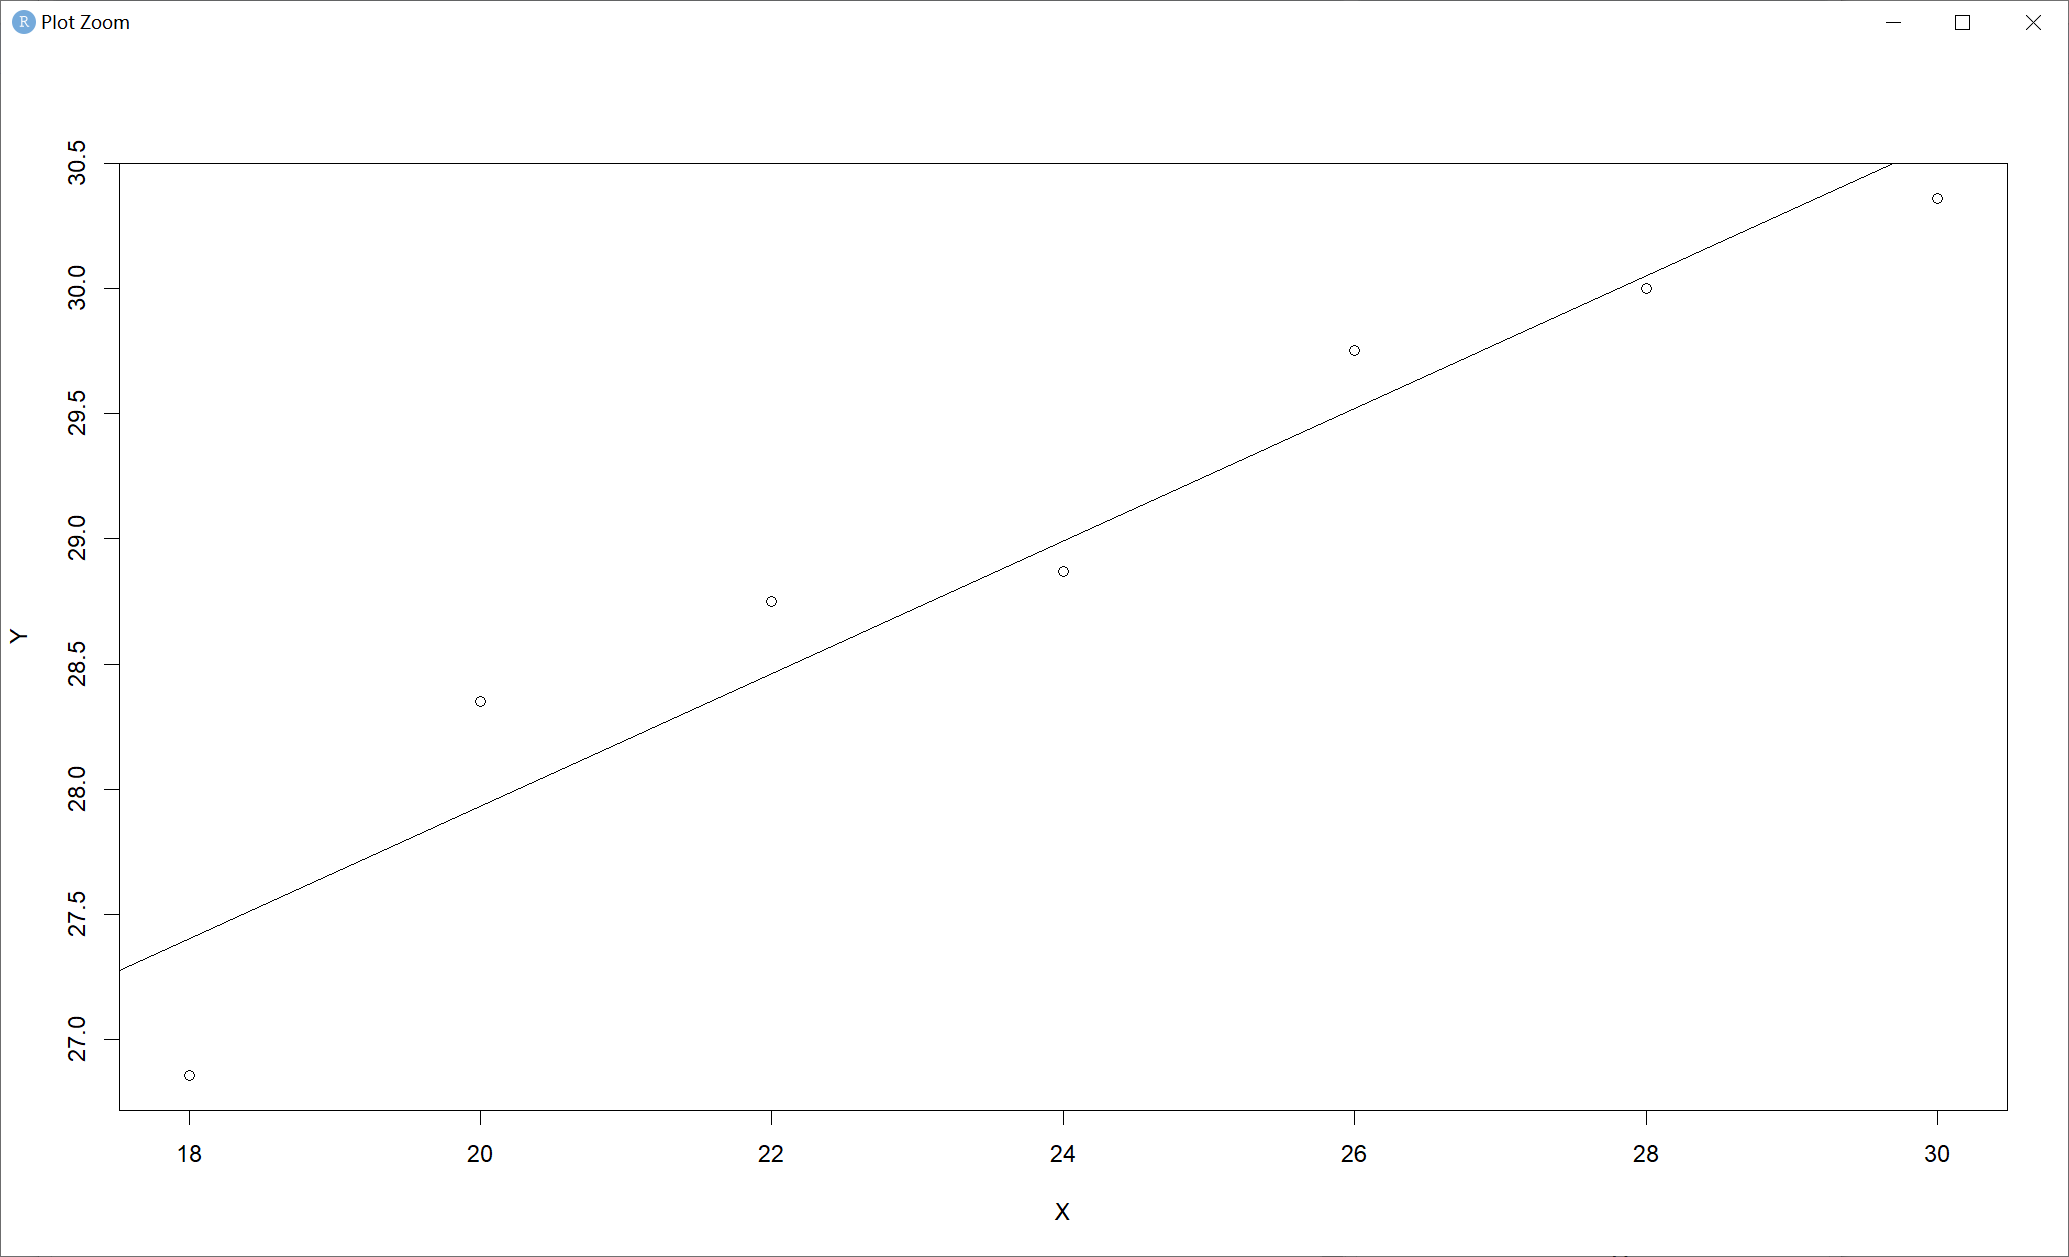
\includegraphics[width=26em]{image/ex1_plt1.png}
\end{figure}
\begin{homework}
    对于正态线性回归模型
\[\bm y=X\bm \beta +e, \qquad e \sim N(0,\sigma^2 I_n)\]
给出参数向量$\beta$的极大似然估计,并与OLS比较。
\end{homework}
\begin{proof}[\solutionname]
    参数向量$\bm \beta$的似然函数:
    $$
    L(\bm \beta )=(2\pi \sigma^2)^{-\frac{n}{2}} exp\{-\frac{1}{2\sigma^2}(\bm y-X\bm \beta)^T(\bm y-X\bm \beta)\}
    $$
    求解似然函数$L(\bm \beta)$的最大值等价于求解如下函数的最小值:
    $$
    Q(\bm \beta) = (\bm y-X\bm \beta)^T(\bm y-X\bm \beta)
    $$
    对$\bm \beta$求导,并令导数为0,得:
    $$
    \dfrac{\p Q}{\p \bm \beta}=2X^T(X\bm \beta -\bm y)
    $$
    故$\hat{\bm \beta}_{MLE}=(X^TX)^{-1}X^T\bm y$.

    证明上述$\hat{\bm \beta}_{MLE}$确实使$Q(\bm \beta)$达到最小值。一种方法是验证Hessian矩阵$\dfrac{\p^2 Q}{\p \bm \beta \bm \beta^T}=2X^TX$为半正定矩阵。另一种方法是:
    $$
    \begin{aligned}
         Q(\bm \beta) &= \Vert \bm y-X\bm \beta \Vert_2^2 \\
         &= \Vert \bm y- X\hat{\bm \beta}_{MLE} + X\hat{\bm \beta}_{MLE} -X\bm \beta \Vert_2^2 \\
         &= \Vert \bm y- X\hat{\bm \beta}_{MLE} \Vert_2^2 + \Vert X\hat{\bm \beta}_{MLE} -X\bm \beta \Vert_2^2 + (\bm y- X\hat{\bm \beta}_{MLE})^T(X\hat{\bm \beta}_{MLE} -X\bm \beta) \\
         &= \Vert \bm y- X\hat{\bm \beta}_{MLE} \Vert_2^2 + \Vert X\hat{\bm \beta}_{MLE} -X\bm \beta \Vert_2^2 \\
         &\geq \Vert \bm y- X\hat{\bm \beta}_{MLE} \Vert_2^2
    \end{aligned}
    $$
    其中等式第三行最后一项为0。故$\hat{\bm \beta}_{MLE}$确实使$Q(\bm \beta)$达到最小值。

    参数向量$\bm \beta$的极大似然估计与OLS估计的结果是一样的。
\end{proof}
\begin{note}
    求导并令导数为0后需进一步验证$\hat{\bm \beta}_{MLE}$确实使$Q(\bm \beta)$达到最小值。注意到求解过程实际在求$\min_{\bm \beta} (\bm y-X\bm \beta)^T(\bm y-X\bm \beta)$,与OLS目标相同。若$X^TX$不可逆就用广义逆代替。
\end{note}

\begin{homework}
    对于简单线性回归模型$Y=\beta_0+\beta_1X+e$,考虑回归变量为随机变量。假设$(x_1,y_1),\dots,(x_n,y_n)\quad i.i.d. \sim N(\mu, \Sigma)$,其中
    \[
    \mu=\begin{bmatrix}
        \mu_x\\
        \mu_y
    \end{bmatrix}
    \quad
    \Sigma=\begin{bmatrix}
        \sigma_x^2 & \rho\sigma_x\sigma_y\\
        \rho\sigma_x\sigma_y & \sigma_y^2
    \end{bmatrix}
    \]
    请给出$\beta_1$关于$\mu,\Sigma$的表达式,并给出$\rho $的一个估计量。
\end{homework}
\begin{proof}[\solutionname]
\[
    \rho\sigma_x\sigma_y=\Cov(X,Y)=\Cov(X,\beta_0+\beta_1X+e)=\beta_1\Cov(X,X)=\beta_1\sigma_x^2 \Rightarrow \beta_1=\rho\frac{\sigma_y}{\sigma_x}
    \]
    取Pearson相关系数作为$\rho$估计:$r=\hat{\beta_1}\dfrac{\hat{\sigma_x}}{\hat{\sigma_y}}=\dfrac{SXY}{\sqrt{SXX\cdot SYY}}$
\end{proof}
\begin{note}
    这里是总体模型,注意区分参数和估计量。
\end{note}
\end{document}